\documentclass{ip-lab}

\labtype{Nivel 4}
\labnumber{Laboratorio 3}
\labtitle{Matrices y análisis de datos}

\makeheader

\begin{document}

\maketitle

\begin{sectionbox}{Objetivos}
\begin{enumerate}
    \item Manipular matrices representando información estructurada.
    \item Visualizar y analizar datasets usando Pandas y Matplotlib.
\end{enumerate}
\end{sectionbox}

\begin{sectionbox}{Preparación del ambiente de trabajo}
Para este laboratorio debe crear dos módulos: \texttt{matrices.py} para las actividades de matrices y \texttt{analisis\_musica.py} para las actividades de visualización. 

Se le proporcionará un archivo \texttt{cupicharts.csv} con datos de canciones en las listas de popularidad.
\end{sectionbox}

\pagebreak

\section{Parte 1: Matrices}

\begin{sectionbox}{Actividad 1: Búsqueda en cuadrantes}

Escriba una función que reciba una matriz cuadrada de enteros positivos y el nombre de un color. El color determina en qué cuadrante de la matriz se debe buscar. La función debe retornar el primer número en el cuadrante especificado que sea par, cuando se recorra por filas y luego por columnas. Si no existe tal número, debe retornar \texttt{None}.

La matriz se divide en seis cuadrantes nombrados por colores:

\textbf{Mitad superior de la matriz:}
\begin{itemize}
    \item \textbf{Rojo:} tercio izquierdo de columnas
    \item \textbf{Verde:} tercio central de columnas
    \item \textbf{Azul:} tercio derecho de columnas
\end{itemize}

\textbf{Mitad inferior de la matriz:}
\begin{itemize}
    \item \textbf{Amarillo:} tercio izquierdo de columnas
    \item \textbf{Naranja:} tercio central de columnas
    \item \textbf{Morado:} tercio derecho de columnas
\end{itemize}

\begin{center}
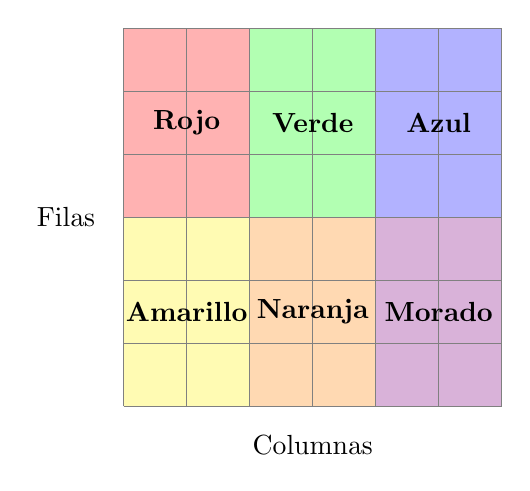
\begin{tikzpicture}[scale=0.8]
    % Draw grid
    \draw[step=1cm,gray,very thin] (0,0) grid (6,6);
    
    % Fill quadrants with colors
    \fill[red!30] (0,3) rectangle (2,6);
    \fill[green!30] (2,3) rectangle (4,6);
    \fill[blue!30] (4,3) rectangle (6,6);
    \fill[yellow!30] (0,0) rectangle (2,3);
    \fill[orange!30] (2,0) rectangle (4,3);
    \fill[violet!30] (4,0) rectangle (6,3);
    
    % Draw grid again on top
    \draw[step=1cm,gray] (0,0) grid (6,6);
    
    % Labels
    \node at (1,4.5) {\textbf{Rojo}};
    \node at (3,4.5) {\textbf{Verde}};
    \node at (5,4.5) {\textbf{Azul}};
    \node at (1,1.5) {\textbf{Amarillo}};
    \node at (3,1.5) {\textbf{Naranja}};
    \node at (5,1.5) {\textbf{Morado}};
    
    % Axis labels
    \node[below] at (3,-0.3) {Columnas};
    \node[left] at (-0.3,3) {Filas};
\end{tikzpicture}
\end{center}

\textbf{E.g.:} En una matriz 6x6, el cuadrante verde abarca las filas 0-2 y columnas 2-3.

\end{sectionbox}

\pagebreak

\begin{sectionbox}{Actividad 2: Modificación de patrones}

Escriba una función que reciba una matriz cuadrada y la modifique pintando la letra "T".

\begin{itemize}
    \item La primera fila de la matriz debe contener únicamente el carácter \texttt{-}
    \item La columna del medio debe contener el carácter \texttt{|} desde la segunda fila hasta la última fila
    \item Todas las demás posiciones de la matriz deben contener el carácter espacio \texttt{' '}
\end{itemize}

Ejemplo para una matriz 5x5:

\begin{center}
\includegraphics[width=0.4\textwidth]{matrix_t.png}
\end{center}

\end{sectionbox}

\pagebreak

\begin{sectionbox}{Actividad 3: Análisis de datos estructurados}

Escriba una función que reciba una tupla con información de ventas y el nombre de una ciudad, y retorne una tupla con el producto que tiene mayores ventas en esa ciudad y el valor de esas ventas.

La tupla de información contiene tres elementos:
\begin{itemize}
    \item Una matriz donde cada fila representa un producto y cada columna representa una ciudad
    \item Una lista con los nombres de los productos (en el mismo orden que las filas)
    \item Una lista con los nombres de las ciudades (en el mismo orden que las columnas)
\end{itemize}

Si la ciudad especificada no existe en los datos, la función debe retornar la tupla \texttt{(None, None)}.

\textbf{E.g.:} Si la matriz es \texttt{[[1500, 2000], [800, 1500]]}, los productos son \texttt{["Laptop", "Mouse"]}, las ciudades son \texttt{["Bogotá", "Medellín"]}, y se consulta por \texttt{"Medellín"}, la función debe retornar \texttt{("Laptop", 2000)} porque 2000 es mayor que 1500.

\end{sectionbox}

\pagebreak

\begin{sectionbox}{Actividad 4: Simulación de salón de clase}

Escriba una función que reciba una matriz cuadrada representando un salón de clase y retorne las coordenadas del primer estudiante introvertido que empezará a hablar en clase. Si ningún introvertido empezará a hablar, debe retornar \texttt{(None, None)}.

En la matriz, cada posición puede contener:
\begin{itemize}
    \item \texttt{0}: Puesto vacío
    \item \texttt{1}: Estudiante introvertido (callado)
    \item \texttt{2}: Estudiante extrovertido (hablando)
\end{itemize}

Un estudiante introvertido empezará a hablar si cumple estas dos condiciones simultáneamente:
\begin{enumerate}
    \item Tiene estudiantes extrovertidos en las dos posiciones diagonales inmediatamente detrás de él (diagonal inferior izquierda y diagonal inferior derecha). Si alguna de estas diagonales no existe porque el estudiante está en el borde del salón, esta condición no se cumple.
    \item La posición inmediatamente adelante no contiene un estudiante extrovertido. Si la posición adelante no existe porque el estudiante está en la primera fila, esta condición sí se cumple.
\end{enumerate}

El recorrido debe realizarse de adelante hacia atrás (de arriba hacia abajo) y de izquierda a derecha, como si estuviera mirando el salón desde el tablero.

E.g.: Si hay un introvertido en posición (1,1), tiene extrovertidos en (2,0) y (2,2), y la posición (0,1) no contiene un extrovertido, entonces ese introvertido empezará a hablar y sus coordenadas deben ser retornadas.

\end{sectionbox}

\pagebreak

\section{Parte 2: Visualización de datos con Pandas}

\begin{sectionbox}{Actividad 5: Análisis de popularidad musical}

Escriba un programa que cargue el archivo \texttt{cupicharts.csv} usando Pandas y genere dos gráficas de análisis sobre las canciones en las listas de popularidad.

\textbf{Gráfica 1: Distribución de canciones por género para un artista}

Implemente una función que reciba el DataFrame y el nombre de un artista, filtre las canciones de ese artista, y genere una gráfica de barras verticales mostrando cuántas canciones tiene en cada género musical.

La gráfica debe incluir:
\begin{itemize}
    \item Título indicando el nombre del artista
    \item Etiqueta del eje X: ``Género''
    \item Etiqueta del eje Y: ``Cantidad de canciones''
\end{itemize}

\begin{center}
\includegraphics[width=0.7\textwidth]{by_genre.png}
\end{center}

\textbf{Gráfica 2: Popularidad total por género para un nivel de explicitidad}

Implemente una función que reciba el DataFrame y un valor booleano indicando si se quieren analizar canciones explícitas o no explícitas. La función debe filtrar las canciones según ese criterio, agrupar por género, sumar la popularidad total de cada género, ordenar de mayor a menor, tomar los 20 géneros más populares, y generar una gráfica de barras horizontales.

La gráfica debe incluir:
\begin{itemize}
    \item Título indicando si son canciones explícitas o no explícitas
    \item Etiqueta del eje X: ``Popularidad total''
    \item Etiqueta del eje Y: ``Género''
    \item El eje Y invertido para mostrar el género más popular en la parte superior
    \item Solo los 20 géneros con mayor popularidad total
\end{itemize}

\begin{center}
\includegraphics[width=0.7\textwidth]{popular_genres.png}
\end{center}

\end{sectionbox}

\pagebreak

\begin{sectionbox}{Entrega}

Entregue un archivo comprimido (ZIP) que contenga:

\begin{enumerate}
    \item \textbf{matrices.py}: Implementación de las Actividades 1-4
    \item \textbf{analisis\_musica.py}: Implementación de la Actividad 5
\end{enumerate}

Suba el archivo comprimido a través de Brightspace en el laboratorio del Nivel 4 designado como ``N4-L3: Matrices y análisis de datos''.

\end{sectionbox}

\end{document}

